\documentclass{article}

% Use the neurips_2026 style file provided
\usepackage{neurips_2026}
\usepackage[utf8]{inputenc}
\usepackage[T1]{fontenc}
\usepackage{hyperref}
\usepackage{url}
\usepackage{booktabs}
\usepackage{amsfonts}
\usepackage{nicefrac}
\usepackage{microtype}
\usepackage{xcolor}
\usepackage{amsmath}
\usepackage{graphicx}
\usepackage{multirow}
\usepackage{tikz}
\usetikzlibrary{arrows.meta,shapes.geometric,shapes.symbols}


\title{Beyond the Next Token: Latent Execution-Graph Retrieval for Agentic Planning}

% \title{LEGR: Latent Execution-Graph Retrieval for Agentic Planning}
\author{%
  Tanay Kadam \\
  North Carolina State University, Lenovo \\
}

\begin{document}

\maketitle
\begin{abstract}
Mapping natural-language requests to executable tool workflows (which we call \emph{intent mapping}) is a bottleneck in agentic systems. Two brittleness modes recur: semantic drift during single-tool selection, and edge hallucination during multi-step planning. We address each with a decoupled retriever. For single-tool selection, we pair a zero-shot LLM router with a \emph{Functional Categorization}, a scheme that groups tools by \emph{action type} rather than domain topic; this training-free single-tool retriever improves routing accuracy by up to 18.5 percentage points under lexical variation. For multi-step planning, we replace autoregressive plan generation ($\mathcal{O}(N)$ sequential decoding, prone to structural edge hallucination) with \textbf{Latent Execution-Graph Retrieval (LEGR)}, a dual-encoder model that retrieves an execution DAG from a pre-indexed corpus and is trained with a graph-aware contrastive objective regularized by graph edit distance. On benchmarks derived from ToolBench and BFCL, LEGR retrieves the correct DAG on a held-out topology family (Diamond) with Recall@1 of 0.963. Because retrieval cost depends on corpus size and not plan size, LEGR's mean latency stays flat at 4.39\,ms, roughly $400$--$625\times$ below the two autoregressive LLM baselines we compare against. Code and data: \href{https://github.com/tanay-kadam/LEGR}{LEGR}.
\end{abstract}

\begin{figure*}[t]
\centering
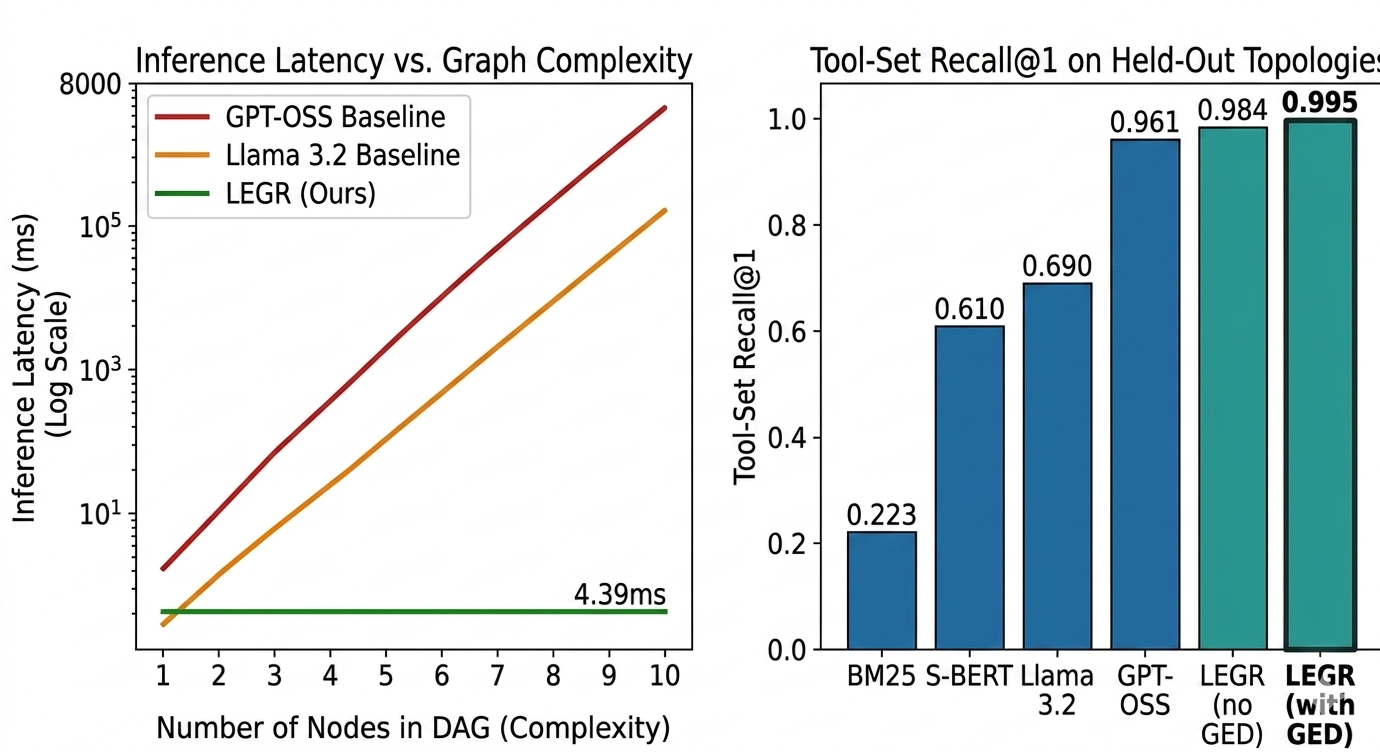
\includegraphics[width=\textwidth]{results.png}
\caption{\textbf{Core LEGR Results and Scalability Analysis.} \textbf{(Left) Inference Latency vs. Graph Complexity.} Autoregressive LLM baselines exhibit linear latency growth as the execution DAG grows (more tool nodes to describe). LEGR performs a single nearest-neighbor lookup and its latency is independent of plan size, staying flat at 4.39\,ms. \textbf{(Right) Retrieval Accuracy on Held-Out (OOD) Topologies.} Recall@1 comparison on the \textit{test\_topology\_heldout} split. LEGR outperforms lexical (BM25) and dense (Sentence-BERT) baselines, and the GED-weighted loss further improves structural alignment.}
\label{fig:results}
\end{figure*}

\section{Introduction}

Tool-augmented LLMs rely on \emph{intent mapping} to translate user requests into appropriate tools and valid \emph{execution structures} (e.g., directed acyclic graphs, DAGs) that respect data dependencies \cite{mialon2023augmented,shen2023hugginggpt,song2023restgpt}. This translation must be precise: selecting a tool with an incorrect action type (e.g., a write instead of a read) can create unintended side effects, and inaccurate edges can corrupt downstream inputs.

Agentic systems struggle with intent mapping in two ways. \textbf{(1) Semantic drift in single-tool selection.} Tools are commonly exposed under human-friendly topic categorizations (e.g., HR, Finance) or domain-specific semantic splits (e.g., chemistry/biology \cite{ding2025scitoolagent}). Topic labels are unreliable proxies for a tool's function when sibling tools share nouns but differ in side effects, so tool retrievers overfit to topical keywords and become brittle under paraphrasing or lexical variation. \textbf{(2) Edge hallucination in multi-step planning.} For multi-step tasks, even recent graph-augmented planners \cite{chen2026gtool,xiu2026optgraph} let an LLM serialize plans token by token, so latency scales linearly with plan size and validation-guided repair cycles are often needed to fix hallucinated dependency edges.

We address these two sub-problems with two decoupled retrievers dispatched by a task-complexity gate (see \S\ref{sec:overview}): atomic single-tool requests are handled by a training-free single-tool retriever built on Functional Categorization; multi-step requests are handled by LEGR. We deliberately decouple the paths because a wrong atomic-selection decision propagates as a silent structural error through every downstream edge of a compounded plan; the tradeoff is that the two paths do not share evidence at inference, which we revisit in \S6. Our contributions are:
\begin{itemize}
    \item We propose a training-free \textbf{single-tool retriever} built on a \textbf{Functional Categorization} (tools grouped by action type rather than domain topic), which mitigates semantic drift and improves routing accuracy by up to 18.5 percentage points under lexical variation at the 15-tool scale.
    \item We introduce \textbf{Latent Execution-Graph Retrieval (LEGR)} for multi-step planning, formulating tool orchestration as dual-encoder DAG retrieval. Planning latency depends on corpus size rather than plan size (unlike the $\mathcal{O}(N)$ sequential decoding of autoregressive planners), giving 4.39\,ms mean latency and roughly two orders of magnitude speedup over the autoregressive baselines we compare against (Figure~\ref{fig:results}).
    \item We propose a contrastive loss regularized by Graph Edit Distance (GED) to enforce topological awareness in the latent space, mitigating edge hallucinations.
    \item We release a benchmark derived from ToolBench and BFCL, demonstrating LEGR's structural generalization to unseen topologies (Recall@1 of 0.963).
\end{itemize}

\begin{figure*}[t]
\centering
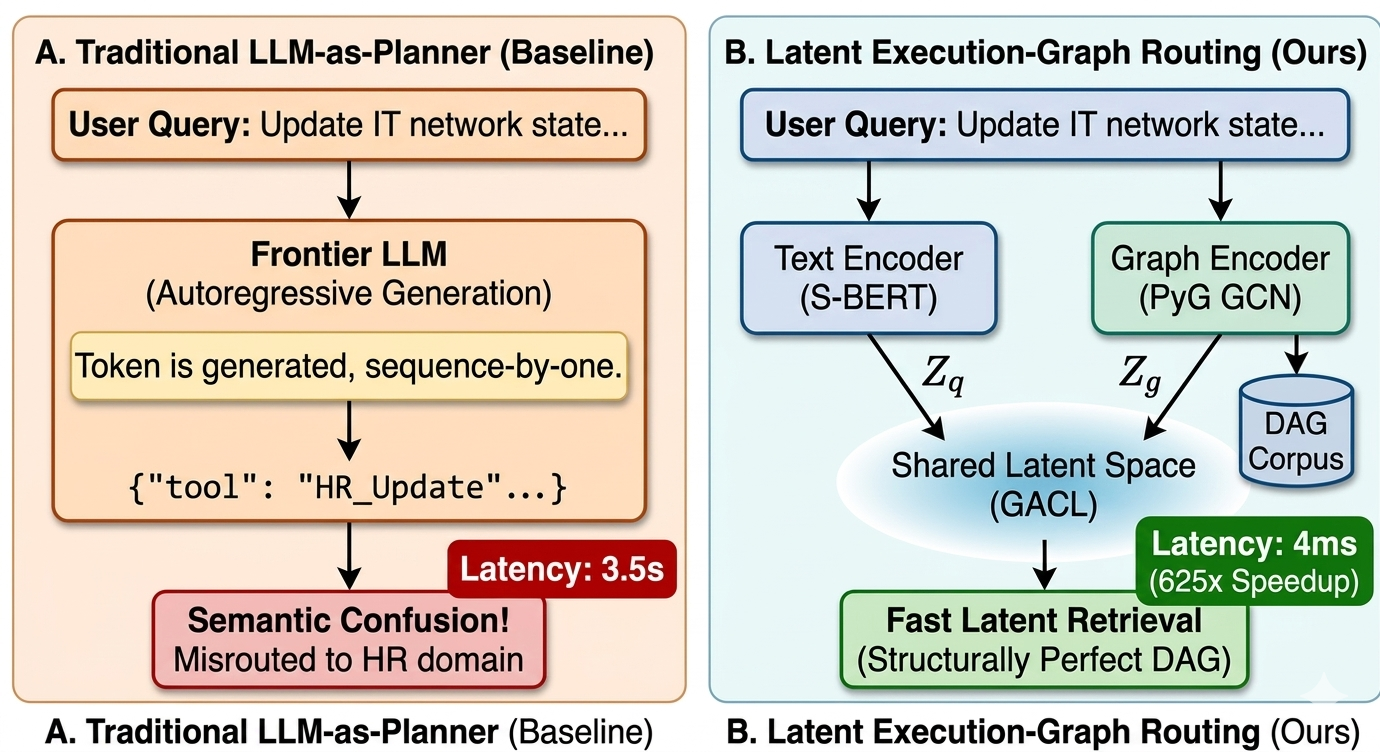
\includegraphics[width=\textwidth]{legr.png}
\caption{\textbf{Teaser.} Comparison between a traditional autoregressive LLM tool planner and our proposed Latent Execution-Graph Retrieval (LEGR). Left: token-level planning can topically drift and misroute requests to the wrong topic. Right: LEGR directly retrieves the correct execution DAG in a shared latent space, yielding much lower latency.}
\label{fig:teaser}
\end{figure*}

\section{Background and Related Work}

\textbf{Single-tool selection and semantic drift.} Tool-augmented LLMs can emit syntactically valid tool invocations \cite{schick2023toolformer,patil2023gorilla} and are evaluated by benchmarks such as ToolBench \cite{qin2023toolllm} and BFCL \cite{yan2024berkeley}, with agent frameworks such as AutoGen \cite{wu2023autogen} formalizing agent--tool interactions. In deployment, tools are typically exposed through \emph{topic categorizations} (e.g., HR, Finance) or domain-specific semantic splits (e.g., SciToolAgent's chemistry/biology categorization \cite{ding2025scitoolagent}). Such labels do not always separate operationally distinct actions (e.g., a read vs.\ a write) that share nouns, leaving routers vulnerable to lexical shifts and ``confusable siblings.'' We instead group tools by \emph{action class} (read, write, orchestrate) and use this Functional Categorization inside a zero-shot LLM router, aligning the routing boundary with system-side risk rather than domain topic.

\textbf{Generative and graph-augmented planning.} Multi-step tool use requires producing an \emph{execution structure} that captures dependencies. The dominant approach serializes a workflow textually and lets an LLM emit it token by token (e.g., ReAct \cite{yao2022react}, DSPy \cite{khattab2023dspy}). Recent graph-augmented frameworks such as GTool \cite{chen2026gtool}, OptGraph \cite{xiu2026optgraph}, and TGR \cite{gao2025tool} narrow the modality gap by feeding graph tokens or validation feedback back into the LLM, but they remain autoregressive: decoding $N$ tokens takes $N$ sequential passes, scaling latency as $\mathcal{O}(N)$, and typically still requires validation-guided repair loops to fix edge hallucinations. GTool trains a missing-dependency predictor (MDPL) and TGR uses a gatekeeping discriminator, but both keep the plan itself in the token stream.

\textbf{Retrieval for tool use.} Retrieve-then-generate pipelines fetch candidate APIs with sparse (BM25 \cite{robertson2009probabilistic}) or dense (Sentence-BERT \cite{reimers-gurevych-2019-sentence}) retrievers, then hand the shortlist to a generator. These retrievers treat candidates as flat text and therefore ignore the dependency structure that distinguishes ``the same tools chained'' from ``the same tools fanned out.'' Knowledge-Graph embedding methods (TransE, DistMult) are also not a fit for our setting: they are transductive, score triples inside a single fixed graph, lack a natural-language text encoder, and embed individual nodes rather than whole candidate DAGs. Aligning natural-language intents with executable DAGs directly in a shared latent space remains, to our knowledge, is underexplored. LEGR maps queries and DAGs into a shared space natively and regularizes the space with Graph Edit Distance \cite{sanfeliu1983distance} so that proximity reflects workflow topology.

\section{Methodology}

We formalize intent mapping into two decoupled retrieval tasks: (1) a training-free \emph{single-tool retrieval} step via a \emph{Functional Categorization}, and (2) a dual-encoder model, \textit{Latent Execution-Graph Retrieval} (LEGR), for \emph{multi-step planning} that predicts how tools are composed into an execution DAG.

\subsection{Formalizing Intent Mapping}
\label{sec:overview}
Let $q$ be a user request. Let $\mathcal{T}$ denote the tool library, and let $\mathcal{C} = \{\mathcal{G}_1,\dots,\mathcal{G}_{|\mathcal{C}|}\}$ be a corpus of \emph{candidate execution DAGs} curated offline. Each DAG $\mathcal{G}=(\mathcal{V},\mathcal{E})$ represents a valid multi-tool workflow, where nodes are tool invocations and edges encode data or control dependencies. The goal is to output a workflow $\hat{\mathcal{G}}$ that (i) calls the correct tools and (ii) matches the intended dependency structure.

A recurring source of brittleness in prior systems is that they entangle two distinct design choices:
(i) \textbf{single-tool categorization}: the label space used to organize tools (i.e., the \emph{categorization}); and
(ii) \textbf{workflow planning}: the mechanism that constructs a multi-step execution structure (e.g., a tool chain vs. a fan-out DAG).
We address these separately. First, we define a categorization that better matches tool \emph{action types}. Second, we plan by retrieving an execution DAG.

\paragraph{Framework overview.} Our two solutions are complementary rather than composed. A deployed system uses a lightweight upstream classifier to decide whether an incoming request is \emph{atomic} (a single tool call) or \emph{compositional} (a multi-step workflow), and dispatches it to the single-tool retriever (\S\ref{sec:fc}) or LEGR (\S\ref{sec:legr}) respectively. We treat this task-complexity gate as an interface between the two sub-problems and do not evaluate the gate itself in this work; in practice a keyword heuristic or a short-prompt LLM classifier suffices. Robust handling of the gate's error surface, and the more ambitious step of a fully unified formulation (a single retriever indexing both atomic tools and multi-tool DAGs in one latent space, which would remove the gate entirely) are natural next steps we leave to future work.

\subsection{Sub-Problem 1: Single-Tool Retrieval via Functional Categorization}
\label{sec:fc}
Our single-tool retriever is a two-stage zero-shot LLM router: given a query, it first predicts a top-level category, then predicts the tool within that category. The variable we study is the \textbf{categorization} itself, i.e., the partitioning of the tool library into categories used for routing. We contrast two choices.

\textit{Topic-based Categorization} ($\mathcal{T}_s$) groups tools by topical or organizational subject (e.g., HR, Finance, IT). This can collapse operationally different actions into the same branch: \texttt{reset\_user\_password} (a credential \emph{write}) and \texttt{generate\_access\_report} (a read-only \emph{audit}) both fall under ``Identity Management.'' An LLM router keyed on $\mathcal{T}_s$ can then overfit to topic nouns (``access'', ``identity'') and become brittle under paraphrase, noun omission, or confusable wording.

We instead use a \textit{Functional Categorization} ($\mathcal{T}_f$), which groups tools by \textbf{action type} (the kind of external effect the tool can produce) so the categorization structure reflects the operational decision boundary. Concretely, we use three top-level action classes:
\begin{itemize}
    \item \textbf{State Modification:} state-changing tools (e.g., POST/PATCH requests, credential resets, record updates).
    \item \textbf{Data Retrieval:} idempotent, read-only tools (e.g., GET requests, audit queries, status checks).
    \item \textbf{Orchestration:} meta-tools that manage control flow (e.g., conditional branching, delegation).
\end{itemize}
Structuring the categorization under $\mathcal{T}_f$ reduces reliance on brittle topic vocabulary by emphasizing what the tool \emph{does} (read vs. write vs. control), not what the request \emph{talks about}. Functional Categorization is a scheme, not a model: combined with the two-stage LLM router above, it forms a training-free single-tool retriever. Our comparison in \S\ref{sec:results-fc} runs the identical router over $\mathcal{T}_s$ and $\mathcal{T}_f$, so the label space is the only variable.

\subsection{Sub-Problem 2: Latent Execution-Graph Retrieval (LEGR)}
\label{sec:legr}
LEGR replaces autoregressive plan synthesis with \emph{bi-encoder retrieval} in a shared latent space $\mathbb{R}^d$.

\textbf{Text encoder.} A Transformer encoder $f_\theta(\cdot)$ (\texttt{all-MiniLM-L6-v2}) maps the request $q$ to an embedding $\mathbf{z}_q \in \mathbb{R}^d$.

\textbf{Graph representation.} Each node $v\in\mathcal{V}$ corresponds to a tool invocation (tool name plus a short textual description, when available). We initialize node features from the same text backbone (tool-name and description embeddings) and treat edges $\mathcal{E}$ as directed dependencies.

\textbf{Graph encoder.} A $k$-layer directed Graph Neural Network produces a DAG embedding $\mathbf{z}_g \in \mathbb{R}^d$. Standard GCNs treat edges symmetrically, which would destroy the directed nature of execution graphs (e.g., confusing a read-then-write with a write-then-read). Instead, we use a directed message-passing formulation. For each node $v \in \mathcal{V}$, the representation is updated via:
\begin{equation}
h_v^{(l+1)} = \sigma \left( \text{LN} \left( W_{\text{self}}^{(l)} h_v^{(l)} + \sum_{u \in \mathcal{N}_{\text{in}}(v)} W_{\text{in}}^{(l)} h_u^{(l)} + \sum_{w \in \mathcal{N}_{\text{out}}(v)} W_{\text{out}}^{(l)} h_w^{(l)} \right) \right)
\end{equation}
where $\mathcal{N}_{\text{in}}(v)$ and $\mathcal{N}_{\text{out}}(v)$ are the predecessor and successor nodes of $v$, $\text{LN}$ denotes LayerNorm, and $\sigma$ is the ReLU activation. This is a relational GCN with two edge types (predecessor and successor), so the encoder can distinguish which neighbors sit upstream vs. downstream of $v$ at each layer rather than symmetrizing them as a plain GCN would; combined with pooling, this preserves enough directional information to separate, e.g., a read-then-write from a write-then-read. After $k=3$ layers, we apply global mean pooling and a linear projection to obtain the graph embedding $\mathbf{z}_g = \text{Proj}(\frac{1}{|\mathcal{V}|} \sum_{v \in \mathcal{V}} h_v^{(k)}) \in \mathbb{R}^d$.

\textbf{Inference (retrieval).} Text and graph embeddings are $\ell_2$-normalized ($\hat{\mathbf{z}} = \mathbf{z} / \|\mathbf{z}\|_2$) before comparison, so the dot product below is a cosine similarity. At test time, we retrieve the most compatible workflow from a pre-validated, pre-indexed corpus $\mathcal{C}$:
\begin{equation}
\hat{\mathcal{G}} = \arg\max_{\mathcal{G} \in \mathcal{C}} \; \hat{\mathbf{z}}_q^\top \hat{\mathbf{z}}_g.
\end{equation}
Because all candidate DAG embeddings can be pre-indexed, inference reduces to a single nearest-neighbor lookup. Retrieval cost is $\mathcal{O}(|\mathcal{C}|)$ for exact search and $\mathcal{O}(\log |\mathcal{C}|)$ with standard approximate nearest-neighbor indexing; crucially, it does not grow with the size $N$ of the output plan, unlike the $\mathcal{O}(N)$ sequential decoding of autoregressive planners. This also bypasses downstream validation-guided repair loops.

\begin{figure}[t]
  \centering
  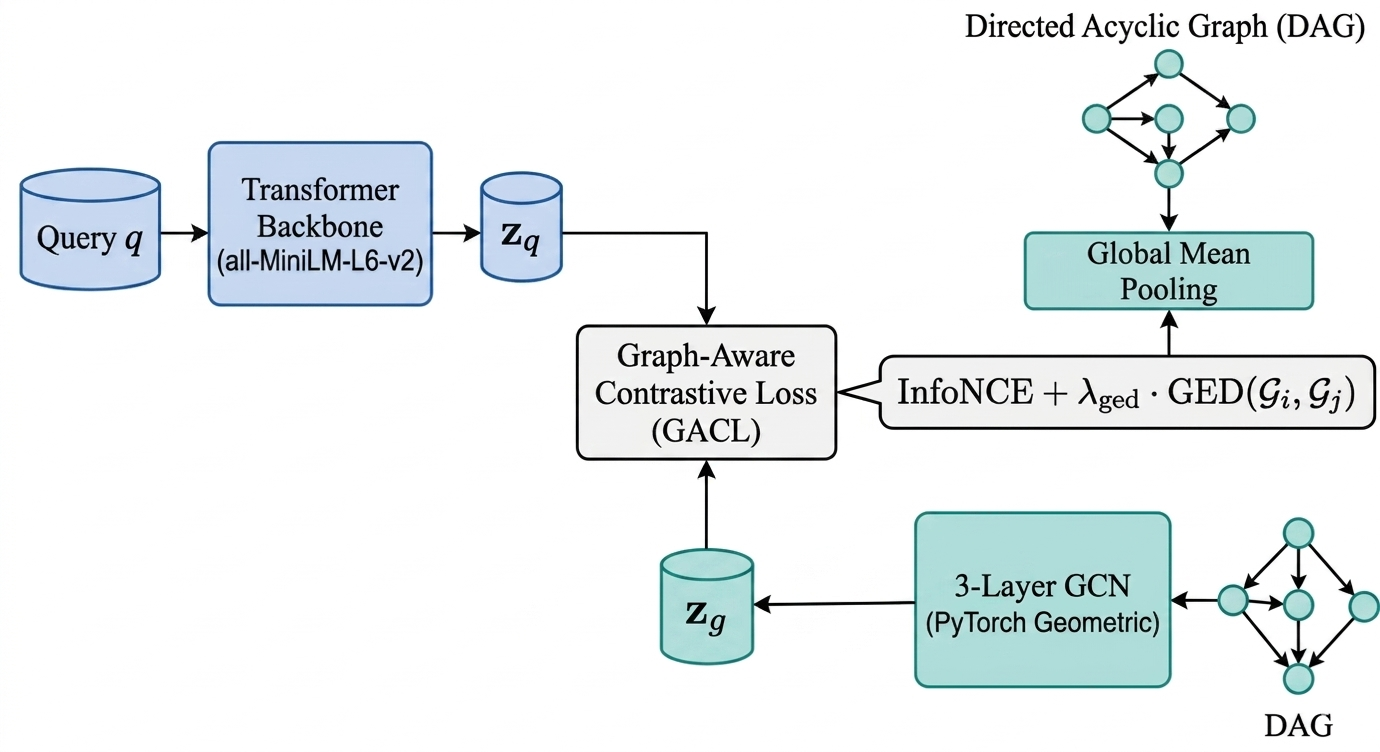
\includegraphics[width=\textwidth]{legr_arch.png}
  \caption{\textbf{Overview of the LEGR Architecture.} Our proposed dual-tower encoder maps natural language queries (Text Tower, Blue) and execution Directed Acyclic Graphs (DAG Tower, Teal) into a shared, topologically informed latent space $\mathbb{R}^d$. The training objective is regularized by the Graph-Aware Contrastive Loss (GACL), which modulates the repulsion strength based on the Graph Edit Distance (GED) between pairs.}
  \label{fig:arch}
\end{figure}

\paragraph{Training objective (GACL).} LEGR is trained to align request and DAG embeddings with a symmetric contrastive objective. Given a batch of $B$ pairs $\{(q_i, \mathcal{G}_i)\}_{i=1}^B$, we form a similarity matrix $\mathbf{S}$ over $\ell_2$-normalized embeddings with entries $\mathbf{S}_{ij} = (\hat{\mathbf{z}}_{q_i} \cdot \hat{\mathbf{z}}_{g_j}) / \tau$, where $\tau$ is a temperature.

Standard InfoNCE implicitly treats all negatives equally. For execution graphs, this is suboptimal: many negatives share the same tool set but differ in a small number of edges, and these ``near-miss'' graphs are the ones a planner must not confuse. We therefore regularize the contrastive loss with Graph Edit Distance (GED) so that negatives with low GED are penalized more strongly.

Concretely, the total loss is:
\begin{equation}
\mathcal{L} = \frac{1}{2} \left( \text{CE}(\mathbf{S}, \mathbf{y}) + \text{CE}(\mathbf{S}^\top, \mathbf{y}) \right) + \lambda_{ged} \cdot \mathcal{L}_{ged}
\end{equation}
where $\text{CE}$ represents the standard cross-entropy loss over the similarity matrix. The structural term is:
\begin{equation}
\mathcal{L}_{ged} = \frac{1}{B} \sum_{i=1}^B -\log \frac{e^{\mathbf{S}_{ii}}}{e^{\mathbf{S}_{ii}} + \sum_{j \neq i} e^{\mathbf{S}_{ij}}(1 - \tilde{w}_{ij})}
\end{equation}
where $\tilde{w}_{ij}$ is a normalized, margin-clamped GED between $\mathcal{G}_i$ and $\mathcal{G}_j$:
\begin{equation}
\tilde{w}_{ij} = \text{clip} \left( \frac{\text{GED}(\mathcal{G}_i, \mathcal{G}_j)}{\text{ged\_scale}} - \text{margin}, 0, 1 \right)
\end{equation}
Because exact GED computation is NP-hard, we pre-compute the pairwise GED matrix for the candidate corpus $\mathcal{C}$ offline using standard approximation heuristics, so this regularization adds no overhead to the training loop. The hyperparameters $\text{ged\_scale}$ and $\text{margin}$ control the penalty threshold. Intuitively, when $\mathcal{G}_j$ is a near-miss of $\mathcal{G}_i$ (low GED) then $\tilde{w}_{ij} \to 0$ and the factor $(1-\tilde{w}_{ij}) \to 1$, so the negative is kept at full strength in the denominator and the loss is pushed to repel it; conversely, when $\mathcal{G}_j$ is structurally distant (high GED) then $\tilde{w}_{ij} \to 1$ and the factor vanishes, so far-away negatives contribute little signal. The latent space is therefore encouraged to organize by \emph{workflow topology} rather than by tool overlap alone.



\section{Dataset and Experimental Setup}

We evaluate two questions: (i) whether \emph{Functional} categorization improves single-tool routing robustness under linguistic shift without training, and (ii) whether LEGR can retrieve the correct \emph{execution DAG} (including edges, not just tool sets) and generalize to unseen workflow \emph{topologies}. To this end, we construct a benchmark of paired natural-language requests and \emph{ground-truth} execution graphs, with controlled topology families and stress-tested query variants.

\subsection{Benchmark Corpus and Held-Out Splits}
We derive the tool vocabulary and natural-language intents from existing tool-use benchmarks (ToolBench \cite{qin2023toolllm} and BFCL \cite{yan2024berkeley}), converting each example into an executable \emph{ground-truth} workflow graph $\mathcal{G}=(\mathcal{V},\mathcal{E})$. To ensure coverage of non-chain structures, we augment the corpus with template-generated DAGs that reuse the same tool library but vary only the dependency pattern. To mitigate dataset-creation bias, the topology templates and linguistic stress variations were generated programmatically using a fixed set of rules prior to model training. For example, synonym substitution was enforced via WordNet \cite{miller1995wordnet}, and graph edges were populated using strict input-output type matching between tools.

We annotate each ground-truth workflow with a \textit{Topology Family} label using simple structural heuristics: \textit{Chain}, \textit{Fan-out}, \textit{Diamond} (edges $0\to1, 0\to2, 1\to3, 2\to3$), and \textit{Hourglass} (edges $0\to2, 1\to2, 2\to3, 2\to4$). To test structural generalization rather than memorization, we adopt a topology-family split. The training split contains only \textit{Chain} and \textit{Hourglass} graphs, while the \textit{Diamond} family is reserved exclusively for evaluation (\texttt{test\_topology\_heldout}). To prevent data leakage, we deduplicate workflows using a hash of the labeled multiset of tool nodes and directed edges. The resulting corpus scales across three tool-vocabulary tiers: the 15-tool setting comprises 3,970 query-graph pairs over 193 distinct DAGs; the 30-tool setting contains 2,060 pairs over 197 DAGs; and the 45-tool setting contains 5,420 pairs over 348 DAGs. Execution graphs range from 1 to 7 nodes, with approximately 300 hard negatives per tier.

\subsection{Linguistic Stress Conditions}
\label{sec:stress}
For categorization-routing experiments, we evaluate under four query conditions designed to isolate common routing failures:
\begin{enumerate}
    \item \textbf{Standard:} original queries with explicit intent.
    \item \textbf{Lexical:} keyword-masked or synonym-substituted queries to reduce noun matching.
    \item \textbf{Confusable:} queries targeting sibling tools with overlapping descriptions but different action types.
    \item \textbf{Paraphrase:} syntactic rephrasings with preserved intent.
\end{enumerate}

\subsection{Baselines and Metrics}
Because there is no established query-to-DAG retriever, we compare LEGR against standard off-the-shelf text retrievers (sparse lexical BM25 and dense Sentence-BERT with the \texttt{all-MiniLM-L6-v2} checkpoint) and against generative LLMs (Llama 3.2 3B~\cite{meta2024llama32} and GPT-OSS 120B~\cite{openai2025gptoss}). For the text retrievers, candidate DAGs are flattened into textual dependency strings (e.g., ``\texttt{tool\_A -> tool\_B}''). For the generative baselines, the model is prompted to autoregressively synthesize the plan as a JSON object listing tools and directed edges. We evaluate the base LLMs directly rather than layering prompting frameworks (e.g., ReAct, ToT) on top, as those frameworks are iterative-reasoning strategies rather than query-to-DAG generation targets. We do not benchmark contemporary graph-augmented planners (GTool~\cite{chen2026gtool}, TGR~\cite{gao2025tool}, OptGraph~\cite{xiu2026optgraph}) directly, because their input formats (dependency-graph triples, gated candidates) and training protocols do not map cleanly onto query-to-DAG retrieval; we discuss them in \S2 as the closest conceptual points of comparison.

For execution-graph retrieval, we report Tool-Set F1, Recall@$k$, and Mean Graph Edit Distance (GED). For categorization routing, we report end-to-end accuracy under each stress condition in \S\ref{sec:stress}.

\subsection{Implementation Details}
\label{sec:impl}
LEGR uses \texttt{all-MiniLM-L6-v2}~\cite{wang2020minilm,reimers-gurevych-2019-sentence} for the text tower and a 3-layer directed GNN with hidden size 256 for the graph tower. Node features are initialized from the same text backbone applied to the tool name and description.

\textbf{Training.} The text tower is partially frozen: the bottom four of MiniLM's six transformer blocks are frozen; the top two blocks, the input embeddings, and the projection head are trained. We optimize with AdamW using a differential learning rate (2e-5 for the trainable backbone; 2e-4 for the projection head, GNN, and $\tau$), weight decay 1e-4, and gradient clipping at 1.0, with a 3-epoch linear warmup followed by cosine decay to 2e-7. Batch size is 128 and max sequence length is 128. Training uses a 100-epoch budget with patience-15 early stopping; runs converged at epoch 56 (30-tool) and epoch 73 (45-tool). The contrastive temperature $\tau$ is learnable, initialized at 0.05, and converges to $\approx 0.030$ (30-tool) and $\approx 0.036$ (45-tool). In Eq.~(4) we set $\text{ged\_scale}=2.5$ and $\text{margin}=0.05$; $\lambda_{ged}=0.10$ at 15 tools and $\lambda_{ged}=0.30$ at 30 and 45 tools. GACL uses in-batch negatives only; the corpus's held-out hard negatives ($\approx 300$ per tier) are used solely at evaluation time. Inside the training loop the GED penalty uses a cheap structural surrogate over the pre-computed pairwise matrix, while all reported Mean GED values use exact \texttt{networkx.graph\_edit\_distance} with unit costs.

\textbf{Hardware and latency protocol.} Local experiments ran on a single laptop (Intel i7-13650HX, 16\,GB RAM, one RTX 4050 6\,GB, PyTorch 2.5.1+cu121); the GPT-OSS 120B baseline was served remotely, so its reported latency includes network round-trip. Retrieval latencies in Table~\ref{tab:retrieval_metrics} measure tokenization plus a forward pass through the text tower at batch size 1 over 100 queries, without warm-up or \texttt{cuda.synchronize()}; nearest-neighbor search is excluded and scales as $\mathcal{O}(|\mathcal{C}|)$ for exact search or $\mathcal{O}(\log|\mathcal{C}|)$ under standard ANN indexing.

\textbf{Evaluation counts.} The four linguistic stress conditions of \S\ref{sec:stress} contain 1005 Standard, 1005 Lexical, 450 Confusable, and 1255 Paraphrase queries at 15 tools. The retrieval evaluation sets contain 1200 queries over 90 DAGs (30-tool tier) and 1100 queries over 78 DAGs (45-tool tier).

For the LLM baselines, both categorization routing and query-to-DAG generation use default sampling with constrained JSON decoding; unparseable outputs and out-of-vocabulary selections are counted as failures. Both categorization schemes (Topic-based and Functional) use identical prompts, isolating the label space as the only independent variable.


\section{Experiments and Results}

We evaluate the two sub-problems in turn: single-tool categorization robustness (\S\ref{sec:results-fc}), execution-graph retrieval (\S\ref{sec:results-legr}), and scaling behavior (\S\ref{sec:results-scale}).

\subsection{Sub-Problem 1: Zero-Shot Categorization Robustness}
\label{sec:results-fc}
Using the two-stage zero-shot routing procedure described in \S\ref{sec:fc}, Table~\ref{tab:routing_results} reports end-to-end accuracy under the four linguistic stress conditions of \S\ref{sec:stress} on the 15-tool library, comparing the two categorization schemes.

\begin{table}[h]
\caption{End-to-End Routing Accuracy (\%) across various linguistic stress conditions.}
\label{tab:routing_results}
\centering
\begin{tabular}{@{}lcccccccc@{}}
\toprule
& \multicolumn{4}{c}{\textbf{GPT-OSS}} & \multicolumn{4}{c}{\textbf{Llama 3.2}} \\
\cmidrule(lr){2-5} \cmidrule(lr){6-9}
Categorization & Std. & Lex. & Conf. & Para. & Std. & Lex. & Conf. & Para. \\
\midrule
Topic-based & 78.3 & 68.1 & 62.7 & 78.0 & 70.0 & 43.3 & 43.3 & 64.9 \\
\textbf{Functional} & \textbf{93.3} & \textbf{75.6} & \textbf{68.0} & \textbf{90.6} & \textbf{83.8} & \textbf{61.8} & \textbf{55.3} & \textbf{79.8} \\
\bottomrule
\end{tabular}
\end{table}

Functional Categorization outperforms Topic-based Categorization on all four conditions and for both routers (Table~\ref{tab:routing_results}). The largest gaps are in conditions where topic nouns are unreliable: under the \textit{Lexical} condition (keyword masking and synonym substitution), Llama 3.2 accuracy rises by 18.5 absolute percentage points (43.3\% to 61.8\%) and GPT-OSS rises by 7.5 points (68.1\% to 75.6\%); the \textit{Confusable} condition shows a similar pattern. This is consistent with the hypothesis that grouping tools by action type (read, write, orchestrate) provides a more reliable zero-shot selection boundary than topical clustering when the surface vocabulary is perturbed.

\textbf{Branching-factor confound.} Functional Categorization uses three top-level branches (Data Retrieval, State Modification, Orchestration), whereas Topic-based Categorization inherits a finer-grained topical partition from the source benchmarks with $K>3$ branches. Part of the accuracy delta may therefore reflect the smaller branching factor rather than the label semantics alone. Two observations argue against a pure branching-factor artifact: (i) the gap widens under \textit{Lexical} and \textit{Confusable} conditions, where topical noun cues are precisely what is removed or disrupted, rather than staying flat as a pure coarseness effect would predict; and (ii) at 30- and 45-tool scales the three-way scheme itself becomes the limiting factor (see ``Categorization Granularity at Scale'' below), consistent with a coarseness--specificity trade-off rather than a monotonic ``fewer branches is better'' effect. We therefore scope the routing claim to the 15-tool, 3-vs-$K$-branch regime and note that hierarchical action categorizations are the principled way to disentangle the two factors.

\subsection{Sub-Problem 2: Execution-Graph Retrieval}
\label{sec:results-legr}
Next, we evaluate LEGR's ability to retrieve the correct execution DAG compared to lexical (BM25) and dense (Sentence-BERT) retrieval baselines, as well as autoregressive generation (Llama 3.2 3B and GPT-OSS 120B). Table~\ref{tab:retrieval_metrics} presents the structural alignment and inference latency on the \textit{test\_topology\_heldout} split (15-tool setting), which exclusively contains Diamond topologies unseen during training.

\textbf{A note on Recall@1 for generative baselines.} Retrieval methods return a ranked list of DAG candidates, so Recall@$k$ is well defined. Generative baselines instead emit a single plan per query and are not ranked. For consistency, we report their Recall@1 as the Tool-Set F1 of the single generated plan; this is why the Tool-Set F1 and Recall@1 entries coincide for the generative rows in Tables~\ref{tab:retrieval_metrics} and~\ref{tab:scalability}. Structural fidelity is captured separately by Mean GED, which does not collapse in this way and remains the primary structural comparison metric.

\begin{table}[h]
\caption{Structural retrieval and latent alignment metrics on the held-out Diamond topology split (15-tool tier). The final column reports each method's mean latency as a multiple of LEGR's: values above $1\times$ are slower than LEGR, values below are faster. $\dagger$~Generative baselines emit a single plan per query rather than a ranked list; we report their Recall@1 as the Tool-Set F1 of that plan (see \S\ref{sec:results-legr}).}
\label{tab:retrieval_metrics}
\centering
\small
\begin{tabular}{@{}lccccc@{}}
\toprule
\textbf{Model} & \textbf{Tool-Set F1} & \textbf{Recall@1} & \textbf{Mean GED $\downarrow$} & \textbf{Latency (ms)} & \textbf{$t/t_{\text{LEGR}}$} \\
\midrule
BM25             & 0.223 & 0.014 & 6.030 & \textbf{0.41} & $0.09\times$ \\
Sentence-BERT           & 0.610 & 0.302 & 4.618 & 9.10 & $2.07\times$ \\
\midrule
LEGR (no GED)    & 0.984 & 0.944 & 0.221 & 4.19 & $0.95\times$ \\
\textbf{LEGR (with GED)} & \textbf{0.995} & \textbf{0.963} & \textbf{0.111} & 4.39 & $1.00\times$ \\
\midrule
Llama 3.2 (Gen)$^\dagger$  & 0.690 & 0.690 & 4.532 & 1,760.0 & $401\times$ \\
GPT-OSS (Gen)$^\dagger$    & 0.961 & 0.961 & 1.590 & 2,742.0 & $625\times$ \\
\bottomrule
\end{tabular}
\end{table}

\textbf{Structural generalization.} LEGR retrieves the correct DAG on the held-out Diamond family at Recall@1 = 0.963 and Tool-Set F1 = 0.995. Sentence-BERT scores Recall@1 = 0.302, showing that a text-only bi-encoder cannot separate topologically distinct graphs that share tool sets. The GED regularizer in GACL closes the remaining structural gap: it halves the Mean GED (0.221 to 0.111) versus the unregularized variant.

\textbf{Inference efficiency.} A single dense retrieval step gives LEGR a mean latency of 4.39\,ms, roughly $401\times$ faster than Llama 3.2 (1,760\,ms) and $625\times$ faster than GPT-OSS (2,742\,ms). Table~\ref{tab:retrieval_metrics} shows a latency--accuracy trade-off among the baselines: BM25 is faster (0.41\,ms) but scores near-zero structural accuracy (Recall@1 = 0.014); GPT-OSS approaches LEGR's tool-set accuracy but takes nearly 3\,s per query. LEGR is the only method in our comparison that avoids this trade-off, and because retrieval cost is a function of corpus size $|\mathcal{C}|$ rather than plan size $N$, its latency stays flat as plans grow (Fig.~\ref{fig:results}, left).

\subsection{Efficiency, Scalability, and Model Footprint}
\label{sec:results-scale}
Table~\ref{tab:model_size} places LEGR next to the baselines on parameter footprint, structural accuracy, and latency.

\begin{table}[h]
\caption{Parameter count, structural accuracy, and latency for all methods. LEGR reduces Mean GED from 1.590 to 0.111 relative to the 120B-parameter autoregressive baseline while running roughly $625\times$ faster.}
\label{tab:model_size}
\centering
\small
\begin{tabular}{@{}llccc@{}}
\toprule
\textbf{Model} & \textbf{Architecture} & \textbf{Parameters} & \textbf{Mean GED $\downarrow$} & \textbf{Latency (ms) $\downarrow$} \\
\midrule
GPT-OSS 120B & Autoregressive LLM & $\approx$ 120.0 Billion & 1.590 & 2,742.00 \\
Llama 3.2    & Autoregressive LLM & $\approx$ 3.2 Billion   & 4.532 & 1,760.00 \\
\midrule
BM25         & Lexical Retrieval  & 0                       & 6.030 & \textbf{0.41} \\
Sentence-BERT       & Dense Retrieval    & $\approx$ 22.7 Million  & 4.618 & 9.10 \\
\textbf{LEGR (Ours)} & \textbf{Sentence-BERT + 3-Layer GNN} & \textbf{$\approx$ 23.5 Million} & \textbf{0.111} & 4.39 \\
\bottomrule
\end{tabular}
\end{table}

LEGR achieves the lowest Mean GED in the table with a total footprint of about 23.5\,M parameters (a 22.7\,M-parameter text backbone and a 3-layer GNN). Relative to the 120B-parameter GPT-OSS baseline, LEGR reduces model size by $\sim 5{,}100\times$, mean inference latency from 2,742\,ms to 4.39\,ms, and Mean GED from 1.590 to 0.111. Accurate multi-tool orchestration therefore does not appear to require a massive autoregressive model in this benchmark; a topology-aware retriever in a properly regularized latent space is sufficient.

\textbf{Scalability and baseline degradation.} We scaled the tool vocabulary to 30 and 45 tools (full results in Appendix~A). LEGR sustains Recall@5 = 1.0 and Tool-Set F1 above 0.987 across all three tool tiers. The baselines degrade: Llama 3.2's Tool-Set F1 drops monotonically from 0.690 (15) to 0.578 (45) and its Mean GED rises from 4.532 to 7.325, indicating trouble synthesizing valid multi-tool plans over a broader action space. Even when autoregressive planners produce the correct tool set, they routinely predict the wrong dependency edges; LEGR sidesteps this \emph{edge hallucination} by retrieving pre-validated execution graphs.

\textbf{Categorization granularity at scale.} While LEGR scales for multi-step planning, the three-way Functional Categorization (read, write, orchestrate) used for single-tool routing becomes under-specified at 30 and 45 tools. Addressing this within-branch confusion calls for a hierarchical categorization, which we identify as future work.

\textbf{Additional analyses.} Detailed ablation studies on the GACL objective (which show that GED weighting is what drives internalization of directed edges), qualitative analyses of the latent space and topic confusion, and a per-case analysis of LEGR's misses versus the generative baselines on the same queries (\S\ref{sec:legr_failures}) appear in the Appendix.


\section{Conclusion}

We decoupled two brittleness modes in agentic intent mapping and treated each as a retrieval problem: semantic drift in single-tool selection is mitigated by a training-free single-tool retriever built on a Functional Categorization (tools grouped by action type), and multi-step edge hallucination is bypassed by LEGR, which retrieves a pre-validated execution DAG rather than autoregressively decoding one. The Functional Categorization retriever improves routing accuracy by up to 18.5 points under lexical stress at the 15-tool scale we evaluated. LEGR, regularized by GACL, retrieves the correct DAG on a held-out topology family (Diamond) with Recall@1 of 0.963 while its latency stays flat with plan size at 4.39\,ms. See \S\ref{sec:results-fc}--\S\ref{sec:results-scale} for the full results and Table~\ref{tab:model_size} for the parameter and latency comparison.

\subsection*{Limitations and Future Work}
Several limitations bound our claims and point to natural next steps.
\textbf{(1) Retrieval is constrained by the pre-indexed corpus.} LEGR can only return workflows present in the offline candidate corpus $\mathcal{C}$; queries that require genuinely novel compositions are outside its scope. We do not measure the cost or coverage properties of curating $\mathcal{C}$, both of which will govern deployment feasibility.
\textbf{(2) The held-out topology evaluation is narrow.} Structural generalization is demonstrated on a single hand-crafted family (Diamond) held out from two others (Chain, Hourglass); real workflows are messier, and stronger structural-generalization claims will require larger and more varied held-out families.
\textbf{(3) Retrieval and generation solve slightly different problems.} By construction, our candidate corpus contains the ground-truth DAG for each evaluation query, whereas the generative baselines must synthesize a DAG from scratch. This is a structural advantage for any retrieval-based method. A natural follow-up is retrieval-augmented generation, in which a generator is conditioned on the top-$k$ retrieved DAGs; we do not evaluate this baseline here.
\textbf{(4) Functional Categorization is coarse at scale.} The three-way scheme becomes under-specified at 30--45 tools (\S\ref{sec:results-scale}); a hierarchical action categorization is a natural remedy.
\textbf{(5) Deployment claims are unverified.} We do not present measurements on edge hardware or under high-throughput serving conditions; the sub-5\,ms latency in our benchmark is suggestive of favorable serving characteristics but is not itself evidence of edge-device viability.
Hybridizing LEGR with a lightweight autoregressive fallback for novel workflows, extending the corpus to cover dynamic, data-dependent control flow, and directly benchmarking against graph-enhanced planners such as GTool and TGR are the primary directions for future work.

\section*{Declaration of LLM Usage}
The authors used Claude 4.7 and Gemini 1.5 Pro for LaTeX formatting, structural organization, and prose refinement. The core methodology, loss function derivation, and experimental execution were developed by the authors.


\nocite{*}

\medskip
\small
\bibliographystyle{unsrt}
\bibliography{references}


\clearpage
\appendix

\section{Scalability to Larger Tool Libraries}

To assess performance as the action space expands, we scaled the tool vocabulary to 30 and 45 tools and evaluated on the held-out Diamond topologies. Table~\ref{tab:scalability} summarizes the retrieval performance across these scales.

\begin{table}[h]
\caption{Scalability of LEGR and baselines across 15, 30, and 45 tools on held-out topologies. LEGR achieves Recall@5 = 1.0 at every scale. $\dagger$~Generative baselines emit a single plan; for these rows Recall@1 is reported as the Tool-Set F1 of that plan (see \S\ref{sec:results-legr}).}
\label{tab:scalability}
\centering
\small
\begin{tabular}{@{}llcccc@{}}
\toprule
\textbf{Tools} & \textbf{Model} & \textbf{Tool-Set F1} & \textbf{Recall@1} & \textbf{Recall@5} & \textbf{Mean GED $\downarrow$} \\
\midrule
\multirow{5}{*}{15}
  & BM25                          & 0.223 & 0.014 & 0.068 & 6.030 \\
  & Sentence-BERT                        & 0.610 & 0.302 & 0.694 & 4.618 \\
  & Llama 3.2 (Gen)$^\dagger$     & 0.690 & 0.690 & ---     & 4.532 \\
  & GPT-OSS (Gen)$^\dagger$       & 0.961 & 0.961 & ---     & 1.590 \\
  & \textbf{LEGR (Ours)}          & \textbf{0.995} & \textbf{0.963} & \textbf{1.000} & \textbf{0.111} \\
\midrule
\multirow{5}{*}{30}
  & BM25                          & 0.150 & 0.012 & 0.056 & 6.358 \\
  & Sentence-BERT                        & 0.531 & 0.316 & 0.663 & 3.811 \\
  & Llama 3.2 (Gen)$^\dagger$     & 0.602 & 0.602 & ---     & 6.903 \\
  & GPT-OSS (Gen)$^\dagger$       & 0.963 & 0.963 & ---     & 1.304 \\
  & \textbf{LEGR (Ours)}          & \textbf{0.997} & \textbf{0.989} & \textbf{1.000} & \textbf{0.038} \\
\midrule
\multirow{5}{*}{45}
  & BM25                          & 0.106 & 0.010 & 0.048 & 9.884 \\
  & Sentence-BERT                        & 0.621 & 0.463 & 0.789 & 3.686 \\
  & Llama 3.2 (Gen)$^\dagger$     & 0.578 & 0.578 & ---     & 7.325 \\
  & GPT-OSS (Gen)$^\dagger$       & 0.959 & 0.959 & ---     & 1.578 \\
  & \textbf{LEGR (Ours)}          & \textbf{0.987} & \textbf{0.975} & \textbf{1.000} & \textbf{0.134} \\
\bottomrule
\end{tabular}
\end{table}

\begin{figure}[htbp]
    \centering
    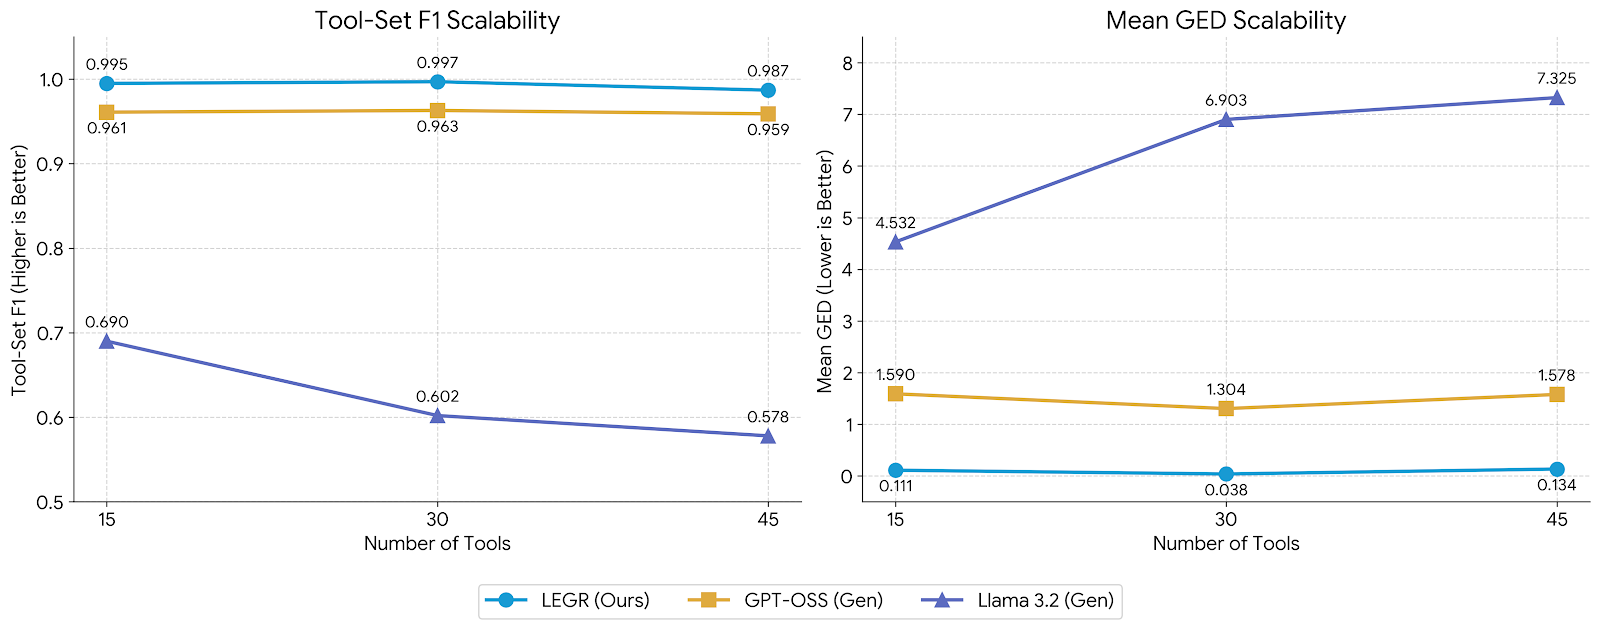
\includegraphics[width=\textwidth]{tool_scale.png}
    \caption{\textbf{Scalability of LEGR compared to Generative Baselines.} Performance across 15, 30, and 45 tools for LEGR, GPT-OSS, and Llama 3.2. \textbf{Left:} Tool-Set F1 score (higher is better). \textbf{Right:} Mean Graph Edit Distance (GED, lower is better). LEGR maintains near-perfect set matching and minimal structural error across all scales. In contrast, Llama 3.2 exhibits a marked degradation in both F1 and GED as the tool space expands.}
    \label{fig:scalability_metrics}
\end{figure}

LEGR sustains Recall@5 = 1.0 and Tool-Set F1 above 0.987 at all three tool counts; Mean GED stays below 0.135. Baseline methods degrade as the vocabulary expands (see the Llama 3.2 rows in particular), consistent with the general pattern that autoregressive generation and lexical matching do not scale in structural fidelity with the action space.

\section{Qualitative Analysis}

\subsection{Mitigating Topic Confusion}
A qualitative review of routing failures under the Topic-based Categorization shows a systematic vulnerability to lexical overlap. The router frequently misclassified ``State Modification'' intents into ``Data Retrieval'' branches when sibling tools shared prominent topic nouns (e.g., \texttt{Update\_User\_Profile} vs. \texttt{Get\_User\_Profile}). Reorganizing the label space around action types largely eliminates this failure mode: the Functional Categorization forces the router to attend to the verb-phrase action rather than the noun-phrase entity.

\begin{figure}[htbp]
  \centering
  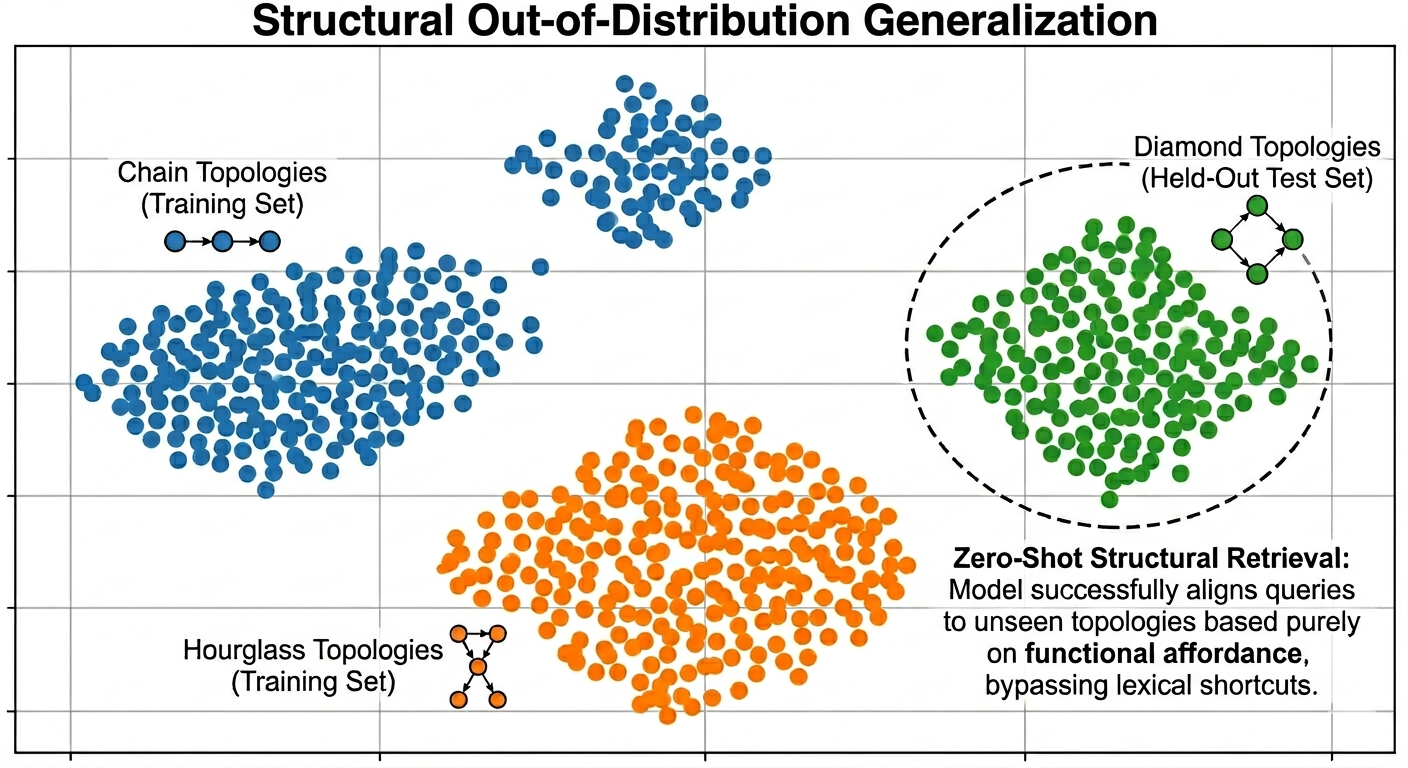
\includegraphics[width=\textwidth]{struct.png}
  \caption{\textbf{Latent Space Topology Visualization.} A 2D projection (t-SNE) of the shared latent space $\mathbb{R}^d$. While the model is trained only on Chain (Blue) and Hourglass (Orange) topologies, it successfully clusters Held-Out Diamond topologies (Green) in a distinct, coherent region. This demonstrates \textbf{Structural Zero-Shot Generalization}.}
  \label{fig:latent_viz}
\end{figure}

\subsection{Structural Zero-Shot Generalization}
LEGR's ability to accurately retrieve "Diamond" topologies, despite only being exposed to "Chain" and "Hourglass" structures during training, demonstrates that the GNN encoder learns a generalizable representation of dependency flow rather than memorizing specific training graphs. Figure~\ref{fig:latent_viz} visualizes a t-SNE projection of the shared latent space, illustrating a clean separation of the held-out Diamond topologies from the training clusters.

\subsection{LEGR Failure Modes}
\label{sec:legr_failures}
We inspected every query on the 15-tool held-out split where LEGR's top-1 retrieval did not match the ground truth (13 cases). In all 13 the ground-truth DAG appears within the top-5, and typically at rank 2: rank 2 in 11 cases, rank 3 in 1, and rank 4 in 1, with a median GED of 3.0 between the top-1 result and the target. This is consistent with the Recall@5 = 1.0 reported in Table~\ref{tab:scalability}. Qualitatively, the misses are near-misses on templates LEGR has already learned: the retrieved DAG has the correct fan-out or hourglass shape but swaps one peripheral tool for a plausible confusable (for example, \texttt{revoke\_access} in place of \texttt{rotate\_api\_key}, or \texttt{escalate\_to\_human} in place of \texttt{send\_notification}).

To check that this subset is genuinely hard (rather than an artifact of the corpus), we re-ran the two generative baselines on the same 13 queries with the identical prompt used in the main experiments. GPT-OSS 120B recovers the exact ground-truth DAG in 8 of 13 cases, with 0 cyclic and 0 parse failures. Llama 3.2 3B reaches 0 exact matches: it emits a cyclic plan in 5 cases and fails to produce parseable JSON in 2. Two observations follow. First, the subset is resolvable, so LEGR's misses are real modelling errors, not label noise. Second, the \emph{quality} of the failures differs sharply: LEGR's worst case is a rank-2 near-miss on a valid, executable DAG, whereas the smaller autoregressive baseline's worst case is a plan that cannot be executed at all.

\section{Ablation of GED Regularization}

We evaluated the necessity of the Graph-Aware Contrastive Loss (GACL) by comparing the full LEGR model ($\lambda_{ged}=0.10$, the value used at the 15-tool tier where Table~\ref{tab:retrieval_metrics} is computed) against an unregularized variant ($\lambda_{ged}=0$). Both variants identify the correct set of tools, but the unregularized model shows a $2.0\times$ degradation in structural alignment: Mean GED rises from 0.111 to 0.221. The GED-weighted denominator is what internalizes the directed edges of the execution DAG, converting a tool-set retriever into an execution-graph retriever.

\end{document}
